Fuzzy sets, as discussed in chapter \ref{ch:intro}, provide a way to encode data. In the case of MCDM  problems, we are particularly interested in modeling the vagueness of fuzzy attributes. And as stated in section \ref{sec:fuzzy_sets} with the set of \emph{tall people}, there is not a unique way to define the membership value of an object to a fuzzy set.\\

Information from three key sources is often considered to define membership functions, and we may exemplify them through the same case of people's height mentioned above: First, concept-driven constraints arise from the inherent nature of what is being modeled (higher heights do not correspond to ''less tall"). Second, domain knowledge or data provides empirical foundations, such as population height statistics, height requirements for particular activities (like basketball), or expert knowledge (the judgement of a basketball coach). Third, the preferences of the decision maker shape the final form, reflecting aspects such as their risk tolerance and the desired level of discrimination between alternatives.\\

% \signal{Define here fuzzification and present what is coming after this.}



% \subsection{Elicitation from Domain Experts}
% \paragraph{Direct elicitation}sfaf



% Another approach that might be more interpretable is:
% \paragraph{Indirect elicitation:}

% Include here linguistic variables:

% 1. Base Variable and Linguistic Values:
% A linguistic variable (e.g., Age) is typically associated with a numerical base variable (e.g., the chronological age from 0 to 100).
% The words or sentences that the linguistic variable can take (e.g., young, old, very young) are its linguistic values.
% A linguistic value like young is interpreted as a label for a fuzzy restriction on the values of the base variable. This fuzzy restriction defines the meaning of the linguistic value.
% 2. Compatibility Function (The Meaning):
% The meaning of a linguistic value is defined by a compatibility function. This function associates each value of the base variable with a number in the interval [0, 1].
% This number represents the compatibility of the numerical value with the linguistic label. For example, the compatibility of the numerical age 28 with the linguistic value young might be 0.7, while the compatibility of age 35 might be 0.2 (p. 4, Fig. 1).
% The paper explicitly states that compatibility is distinct from probability. It is a subjective measure of how well a numerical value fits a linguistic concept.



% \subsection{Learning from data}


% Present this as an optimization subproblem.

% Mention that here you can use labeled data for supervised learning (fitting a function that depends on some parameters via an objective you want to minimize). Even in the case of non labeled data, there exist also unsupervised approaches, for example fuzzy clustering.

% I think ANFIS also would fit into this category.

% As another optimization problem where given a functional form that depends on some parameters you aim to find the function that best



% \subsection{Deriving it from other fuzzy sets}
% Do not mention tarski stuff, omit that.

% Mention fuzzy relational equations

% Mention the use of operators such as AND, OR,... So that from the set of cheap cars and the set of comfortable cars, we may get the set of cheap and comfortable cars.



The process of defining these membership functions is known as fuzzification. Since it is a crucial first step in any fuzzy logic application, the following subsections explore membership function construction methods, which are broadly categorized according to the source of information: elicitation from domain experts, learning from empirical data, or derivation from other pre-existing fuzzy sets.

\subsection{Elicitation from Domain Experts}
An approach to construct membership functions when empirical data is scarce, or the concept being modeled is highly subjective, is to elicit information from domain experts. This process, which can be performed through direct or indirect methods, leverages human knowledge and intuition to quantify vague concepts.

\paragraph{Direct Elicitation}
The most straightforward method is direct elicitation, where an expert is asked to directly assign a numerical membership grade to a series of elements in the universe of discourse. For example, to define the fuzzy set for \emph{high temperature} in a room, the expert could be polled to provide a value between 0 and 1 for several different temperatures. These results form a set of points that define the membership function. For continuous fuzzy sets or cases with too many surveyed points, this approach becomes unfeasible. A key consideration is the scale used for elicitation, which can then be mapped into the $[0,1]$ interval. A common strategy is to use $7\pm2$ categories when making absolute judgements along a single dimension. This idea originated in a psychology paper \cite{miller1956magical}, suggests that simpler scales may be more appropriate than finer ones for elicitation tasks.

\paragraph{Indirect and Compositional Elicitation}
A more interpretable and often more robust approach is indirect elicitation, which avoids requiring experts to provide precise values for each element and instead employs parametrized functional forms. This is commonly achieved through the use of linguistic variables, which provide a formal structure for handling verbal concepts.

\begin{definition}[Linguistic Variable \cite{Zadeh1975}]
A \textbf{linguistic variable} is a variable (e.g., \emph{age}) whose values are words or sentences rather than numbers. It is characterized by a set of linguistic values, or \textbf{terms} (e.g., \emph{young}), defined over an underlying numerical \textbf{base variable} (e.g. a numerical variable \texttt{x} whose values are the integers from 0 to 100). The meaning of each term is captured by a fuzzy set, whose membership function (compatibility function), specifies the degree to which any value on the base variable is compatible with the linguistic label.
\end{definition}

Instead of defining this compatibility function point-by-point, an expert can specify it by choosing a standard, parameterized shape that is easy to interpret. For instance, a triangular fuzzy number is intuitive for representing a concept centered ``around" a certain point, while a trapezoidal shape can represent a concept that is fully valid over an interval. 

Furthermore, new linguistic values can be derived compositionally from existing ones using \emph{linguistic modifiers}, or hedges. These are operations that alter a membership function, such as concentrators like \emph{very}, which makes a fuzzy set more specific, and dilators like \emph{somewhat}, which makes it less specific. These effects are often achieved by applying an exponent to the original membership function: for a concentrator like \emph{very}, the membership values are squared ($\mu_{\text{very } A}(x) = (\mu_A(x))^2$), while for a dilator like \emph{somewhat}, the square root is taken ($\mu_{\text{somewhat } A}(x) = \sqrt{\mu_A(x)}$).

\begin{example}
    Consider the linguistic variable \emph{Price}. An expert might define the term \emph{cheap} as being fully true for prices below \$30 and completely false above \$70. Similarly, the term \emph{expensive} could be defined as false below \$50 and fully true above \$90.
    
    This formulation creates an overlap region (between \$50 and \$70) where an item can be considered, to some degree, \emph{both} cheap and expensive, capturing the inherent ambiguity of mid-range pricing. From these base terms, modifiers like \emph{very} and \emph{somewhat} are used to derive more nuanced linguistic values, as illustrated in Figure \ref{fig:linguistic_variable_overlap}.
\end{example}

\begin{figure}[!ht]
    \centering
    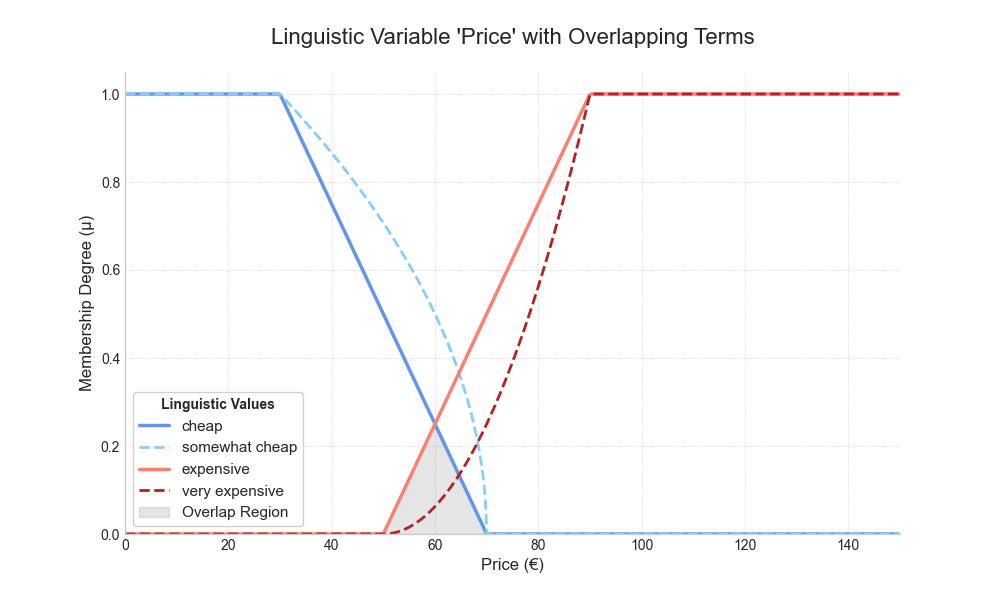
\includegraphics[width=0.8\textwidth]{ch2/figures/fuzzy_var_car_example.png}
    \caption{An illustration of the linguistic variable 'Price' with overlapping terms. The overlap between 'cheap' and 'expensive' represents the ambiguity of mid-range prices. Modifiers create more specific or general terms.}
    \label{fig:linguistic_variable_overlap}
\end{figure}


\subsection{Learning from Data}
When relevant data is available, membership functions can be constructed through learning algorithms. This approach frames the task as an optimization problem, where the goal is to find the membership function that best fit the available data.\\

In a supervised learning context, we have a dataset of input-output pairs. For example, consider a company with data regarding products (e.g. their characteristics) and customer satisfaction surveys. Each product would be an element of the universe and its membership grade is derived from the satisfaction surveys. We can then use function approximation techniques (e.g. Machine Learning models like artificial neural networks), to learn a membership function from the data and use them to generalize to new products with similar characteristics without needing to survey them.\\

In many real-world scenarios, however, we do not have such input-output pairs. For these unsupervised learning contexts, several approaches could be employed, such as fuzzy clustering (which is implemented in the next chapter). This algorithm partitions a dataset into several groups, allowing each data point to belong to multiple clusters with varying degrees of membership. These membership degrees can then be interpreted as the values of the membership function for the fuzzy set represented by each cluster. The Fuzzy C-Means (FCM) algorithm \cite{bezdek1984fcm} stands as the most widely used method in this category.

\paragraph{Fuzzy C-Means (FCM) algorithm} Given a dataset $X = \{x_1, x_2, \ldots, x_n\}$ of $n$ data points in an $r$-dimensional space, FCM aims to find a partition of $X$ into $c$ fuzzy clusters by minimizing the objective function:
\[
J_m(U, V) = \sum_{i=1}^{c} \sum_{k=1}^{n} (u_{ik})^m \|x_k - v_i\|^2
\]
where $U$ is the partition matrix with elements $u_{ik}$ representing the membership of data point $x_k$ in cluster $i$, $V = \{v_1, \ldots, v_c\}$ is the set of cluster centers, and $m > 1$ is a fuzzification parameter that controls the degree of cluster overlap. The minimization of $J_m$ is performed iteratively through the following steps:
\begin{enumerate}
    \item Initialize the partition matrix $U^{(0)}$ randomly, subject to $\sum_{i=1}^{c} u_{ik} = 1$ for each $k$.
    \item At iteration $t$, calculate the cluster centers $V^{(t)}$:
    \[
    v_i^{(t)} = \frac{\sum_{k=1}^{n} (u_{ik}^{(t-1)})^m x_k}{\sum_{k=1}^{n} (u_{ik}^{(t-1)})^m}
    \]
    \item Update the partition matrix $U^{(t)}$:
    \[
    u_{ik}^{(t)} = \left( \sum_{j=1}^{c} \left( \frac{\|x_k - v_i^{(t)}\|}{\|x_k - v_j^{(t)}\|} \right)^{\frac{2}{m-1}} \right)^{-1}
    \]
    \item Repeat steps 2 and 3 until the change in the partition matrix, $\|U^{(t)} - U^{(t-1)}\|$, is smaller than a predefined threshold.
\end{enumerate}
Once the algorithm converges, the resulting column $i$ of the matrix $U$ can be taken as the membership function for the fuzzy set represented by cluster $i$.\\

Memberships decay with the exponent ${-2/(m-1)}$, which provides key insights into the algorithm's operation. When $m$ approaches 1, the exponent approaches negative infinity, causing the nearest center to dominate and resulting in nearly crisp labels. Conversely, as $m$ approaches infinity, the exponent approaches 0, causing distances to lose influence and all memberships to converge to $1/c$. This behavior is clearly illustrated in figure \ref{fig:fuzzy_cmeans}, which shows how different values of $m$ affect the clustering results.

\begin{figure}[!ht]
    \centering
    \begin{adjustwidth}{-1.7cm}{-1cm}
    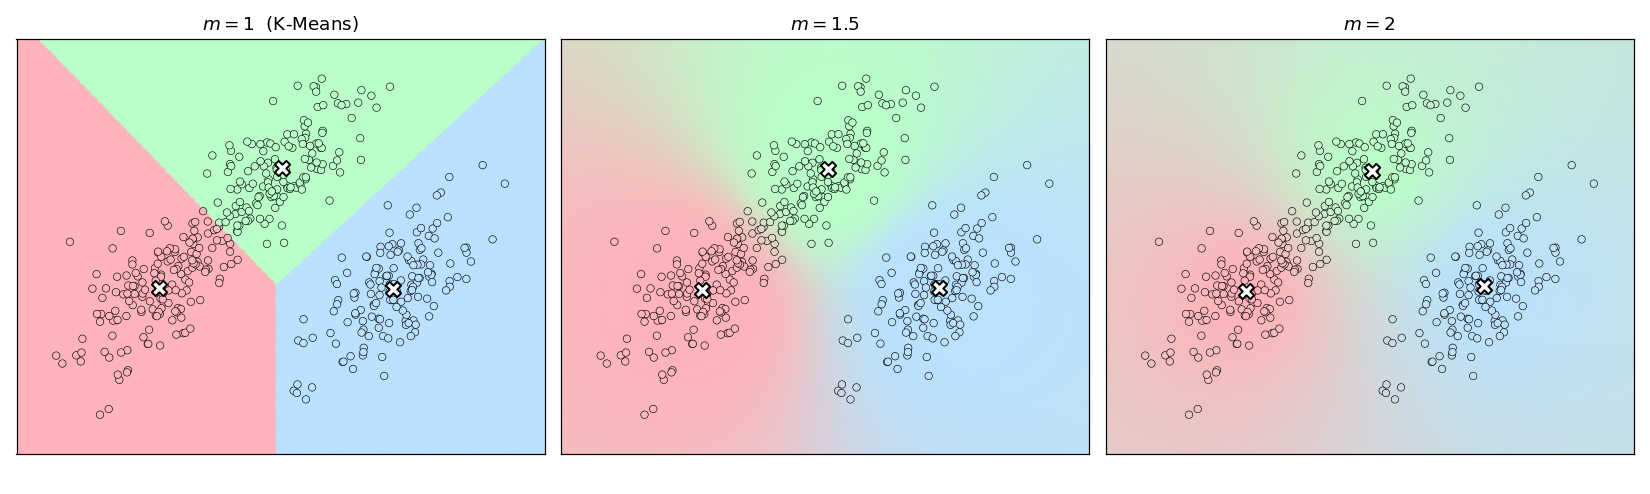
\includegraphics[width=1.15\textwidth]{ch2/figures/fuzzy_cmeans.png}
\end{adjustwidth}
    \caption{3 plots of fuzzy cmeans for 3 clusters with different m values (1, 1.5 and 2). Each color correspond to a cluster whose center is marked with the white cross. Memberships are denoted using gradients of color, where fainter tones denote lower membership values.}
    \label{fig:fuzzy_cmeans}
\end{figure}

\begin{example}
    A marketing firm could use FCM to segment customers based on their purchasing habits (e.g., purchase frequency and average transaction value). The algorithm might identify three clusters, like \emph{Low-Value}, \emph{Medium-Value}, and \emph{High-Value} customers. The membership value $u_{ik}$ would represent the degree to which customer $k$ belongs to the \emph{High-Value} fuzzy set, providing a more nuanced classification than a crisp assignment.
\end{example}

\subsection{Deriving from Other Fuzzy Sets}
New fuzzy sets can also be constructed from existing ones. The most common method is the use of fuzzy set operations (intersection, union and complement), which are particularly useful for creating complex fuzzy concepts from simpler, elementary ones. For instance, if we have already defined membership functions for the fuzzy sets \emph{cheap cars} and \emph{comfortable cars}, we can derive the membership function for \emph{cheap and comfortable cars} by applying a fuzzy AND operator (a t-norm) to the membership values of the original sets.\\

Another, more complex, method involves the use of fuzzy relational equations \cite[Sec.~3.5]{HistoryFL2017}. This approach is typically formulated as an inverse problem. A fuzzy relational equation describes a relationship between two or more fuzzy variables, often in the form $R = P \circ Q$, where $P$ and $Q$ are fuzzy relations and $\circ$ is a composition operator. If two of the three components are known, the third can be determined by solving the equation.

\begin{example}
    In medical diagnosis, let $S$ be a fuzzy relation between patients and symptoms, and $D$ be a fuzzy relation between patients and diseases. These two may be linked through a fuzzy relation $K$ representing medical knowledge, such that $D = S \circ K$. If we have observed data for patients' symptoms $S$ and their final diagnoses $D$, we could solve this equation to infer the underlying medical knowledge relation $K$ that connects symptoms to diseases.
\end{example}